\documentclass[12 pt]{article}
\usepackage[utf8]{inputenc}
\usepackage[english]{babel}
% \usepackage[top=2.5cm, bottom=2.5cm, left=4cm, right=2.5cm]{geometry}
\usepackage{geometry}
 \geometry{
 a4paper,
 % total={210mm,297mm},
 left=40mm,
 right=25mm,
 top=25mm,
 bottom=25mm,
 }
 \usepackage{setspace}
\renewcommand*\abstractname{Abstract}
\usepackage{times}  % Times New Roman
\usepackage{amssymb,amsmath}
\usepackage{ifxetex,ifluatex}
\usepackage{fixltx2e} % provides \textsubscript
\ifnum 0\ifxetex 1\fi\ifluatex 1\fi=0 % if pdftex
  \usepackage[T1]{fontenc}
  \usepackage[utf8]{inputenc}
\else % if luatex or xelatex
  \ifxetex
    \usepackage{mathspec}
    \usepackage{xltxtra,xunicode}
  \else
    \usepackage{fontspec}
  \fi
  \defaultfontfeatures{Mapping=tex-text,Scale=MatchLowercase}
  \newcommand{\euro}{€}
\fi
% use upquote if available, for straight quotes in verbatim environments
\IfFileExists{upquote.sty}{\usepackage{upquote}}{}
% use microtype if available
\IfFileExists{microtype.sty}{\usepackage{microtype}}{}
\usepackage{graphicx}
\makeatletter
\def\maxwidth{\ifdim\Gin@nat@width>\linewidth\linewidth\else\Gin@nat@width\fi}
\def\maxheight{\ifdim\Gin@nat@height>\textheight\textheight\else\Gin@nat@height\fi}
\makeatother
% Scale images if necessary, so that they will not overflow the page
% margins by default, and it is still possible to overwrite the defaults
% using explicit options in \includegraphics[width, height, ...]{}
\setkeys{Gin}{width=\maxwidth,height=\maxheight,keepaspectratio}
\ifxetex
  \usepackage[setpagesize=false, % page size defined by xetex
              unicode=false, % unicode breaks when used with xetex
              xetex]{hyperref}
\else
  \usepackage[unicode=true]{hyperref}
\fi
\hypersetup{breaklinks=true,
            bookmarks=true,
            pdfauthor={Azmi C. Özgen},
            pdftitle={A New Approach to Neural Networks},
            colorlinks=true,
            citecolor=blue,
            urlcolor=blue,
            linkcolor=magenta,
            pdfborder={0 0 0}}
\urlstyle{same}  % don't use monospace font for urls
\setlength{\parindent}{0pt}
\setlength{\parskip}{6pt plus 2pt minus 1pt}
\setlength{\emergencystretch}{3em}  % prevent overfull lines
\setcounter{secnumdepth}{0}

\begin{document}

\pagenumbering{roman}
\onehalfspacing
\pagestyle{plain}
\tableofcontents
\setcounter{page}{1}

\begin{abstract}
    \thispagestyle{plain}
    \pagenumbering{roman}
    \setcounter{page}{2}
    \addcontentsline{toc}
    Machine learning is a growing area in computer science. Neural networks
    is very popular subdomain of it. This project generally covers the work
    of M. Nielsen and his book Neural Networks and Deep Learning{[}1{]}. We
    will first introduce neual networks and then aplly it to a generic
    problem which is called classifying handwritten digits.
\end{abstract}

% \section{1. Abstract}\label{abstract}
%
% Machine learning is a growing area in computer science. Neural networks
% is very popular subdomain of it. This project generally covers the work
% of M. Nielsen and his book Neural Networks and Deep Learning{[}1{]}. We
% will first introduce neual networks and then aplly it to a generic
% problem which is called classifying handwritten digits.

\section{2. Introduction}\label{introduction}

The idea of neural networks is to take a large number of dataset known
as training examples, and then develop a system which can learn from
those training examples. In other words, the neural network uses the
examples to automatically infer rules for recognizing other unknown
examples. Furthermore, by increasing the number of training examples,
the network can learn more about handwriting, and so improve its
accuracy.

There are just 100 training digits below, perhaps we could build a
better handwriting recognizer by using thousands or even millions or
billions of training examples.

\begin{figure}[htp]
\centering
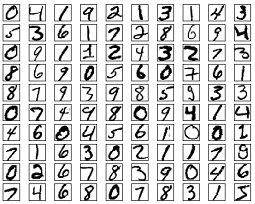
\includegraphics{./figs/mnist_100_digits.png}
\caption{100 Handwritten Digits}
\end{figure}

This project is concerned with write a computer program implementing a
neural network that learns to recognize handwritten digits.

Along the way there are many key ideas about neural networks, including
two important types of artificial neuron (the perceptron and the sigmoid
neuron), and the standard learning algorithm for neural networks, known
as stochastic gradient descent.

\subsection{1.1 Perceptrons}\label{perceptrons}

Perceptron is a type of artificial neuron. Perceptrons were developed in
the 1950s and 1960s by the scientist Frank Rosenblatt, inspired by
earlier work by Warren McCulloch and Walter Pitts. Today, it's more
common to use other models of artificial neurons - in this book, and in
much modern work on neural networks, the main neuron model used is one
called the sigmoid neuron.

A perceptron takes several binary inputs, $ x_1, x_2, \ldots{}, $
and produces a single binary output:

\begin{figure}[htp]
\centering
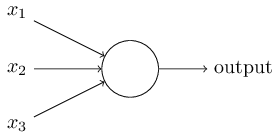
\includegraphics{./figs/tikz0.png}
\caption{Perceptron}
\end{figure}

In general it could have more or fewer inputs. Rosenblatt proposed a
simple rule to compute the output. He introduced weights,
$ w_1,w_2,\ldots{},$ real numbers expressing the importance of the respective
inputs to the output. The neuron's output, 0 or 1, is determined by
whether the weighted sum $ \sum_j w_j x_j $ is less than or
greater than some threshold value. Just like the weights, the threshold
is a real number which is a parameter of the neuron. To put it in more
precise algebraic terms:

\begin{equation}
        output =
        \begin{cases}
            0,& if \hspace{0.5 cm} \sum_j\ w_jx_j \leqslant threshold \\
            1,& if \hspace{0.5 cm} \sum_j\ w_jx_j > threshold
        \end{cases}
\end{equation}

\end{document}
